%************************************************
\chapter{Normalizing Flows}\label{ch:mathtest} % $\mathbb{ZNR}$
%************************************************
\begin{flushright}{\slshape
    Know from the rivers \\
    in clefts and in crevices: \\
    those in small channels flow noisily, \\
    the great flow silent. \\
    Whatever’s not full makes noise.\\
    Whatever is full is quiet. } \\ \medskip
    --- Buddha, Nalaka Sutta
\end{flushright}

In standard probabilistic modeling practice, we represent our beliefs over unknown continuous quantities with simple parametric distributions like the normal, exponential, and Laplacian distributions. However, using such simple forms, which are commonly symmetric and unimodal (or have a fixed number of modes when we take a mixture of them), restricts the performance and flexibility of our methods. For instance, standard variational inference in the Variational Autoencoder uses independent univariate normal distributions to represent the variational family. The true posterior is neither independent nor normally distributed, which results in suboptimal inference and simplifies the model that is learnt. In other scenarios, we are likewise restricted by not being able to model multimodal distributions and heavy or light tails, widespread in HEP.

\emph{Normalizing Flows} are a type of \emph{latent generative model}, capable of producing new, original samples from a latent space, usually a Gaussian one. The main advantage of this approach, when compared to the previous ones, is that it has been specifically engineered to define explicit \emph{densities}--making it particularly well suited to our use case.

The present chapter serves as a general explanation of the basic concepts and ideas for defining and implementing Normalizing Flows (NF for short). We also briefly discuss in a more general way the possible use cases of this architecture. For the interested reader, an excellent review is the one by Papamakarios et al \cite{papanf}.

\section{Definitions}

Normalizing flows are a family of methods for constructing flexible learnable probability distributions, often with neural networks, which allow us to surpass the limitations of simple parametric forms to represent complex high-dimensional distributions.

\subsection{Basics}

The basic idea is to define a complex distribution $p_x(\mathbf{x})$ by passing \emph{random variables} $\mathbf{z} \in \mathbb{R}^D$ drawn from a simple \emph{base distribution} $p_z(\mathbf{z})$ through a non-linear, \emph{invertible} and \emph{differentiable} transformation \emph{f}: $\mathbb{R}^D \rightarrow \mathbb{R}^D$, $\mathbf{x} = f(\mathbf{z})$. \emph{f} can also be called a \emph{bijection}. The base distribution is usually chosen to be simple, for example a standard i.i.d. normal distribution, $\mathbf{z}\sim\mathcal{N}(\mathbf{0},I_{D\times D})$, which makes it very simple to sample and evaluate. 

We may now use the change-of-variable formula to express $p_x(\mathbf{x})$ as:

\[
p_x(\mathbf{x}) = p_z(\mathbf{z})\det\left|\frac{d\mathbf{z}}{d\mathbf{x}}\right|
\]

and remembering that \emph{f} is invertible, taking the logarithm of both sides we get:

\begin{equation}\label{eqn:logpdf}
	\begin{aligned}
		\log(p_x(x)) &= \log(p_z(f^{-1}(\mathbf{x})))+\log\left(\det\left|\frac{d\mathbf{z}}{d\mathbf{x}}\right|\right)\\
		&= \log(p_z(f^{-1}(\mathbf{x})))-\log\left(\det\left|\frac{d\mathbf{x}}{d\mathbf{z}}\right|\right)
	\end{aligned}
\end{equation}

where $d\mathbf{z}/d\mathbf{x}$ denotes the Jacobian matrix of $f^{-1}(\mathbf{x})$, $\mathbb{J}_{f^{-1}}(\mathbf{x})$.
Intuitively, this equation says that the density of $x$ is equal to the density at the corresponding point in $z$ plus a term that corrects for the warp in volume around an infinitesimally small volume around $x$ caused by the transformation.
	We can compose such bijective transformations to produce even more complex distributions. It is clear that, if we have $K$ transforms $f_{(1)}, f_{(2)},\ldots,f_{(K)}$, then the log-density of the transformed variable $\mathbf{x}=(f_{(1)}\circ f_{(2)}\circ\cdots\circ f_{(K)})(\mathbf{z})$ is:
	
	\begin{equation*}
		\begin{aligned}
			\log(p_x(\mathbf{x})) &= \log\left(p_z\left(\left(f_{(K)}^{-1}\circ\cdots\circ f_{(1)}^{-1}\right)\left(\mathbf{x}\right)\right)\right)+\\
			&+\sum^{K}_{k=1}\log\left(\left|\frac{df^{-1}_{(k)}(\mathbf{x}_{(k)})}{d\mathbf{x}'}\right|\right)
		\end{aligned}
	\end{equation*}
	
This relationship between the base distribution and the transformed one through this chain of invertible transforms is at the core of the NF approach and is illustrated in Figure \ref{fig:nf}.

\begin{figure}
    \centering
    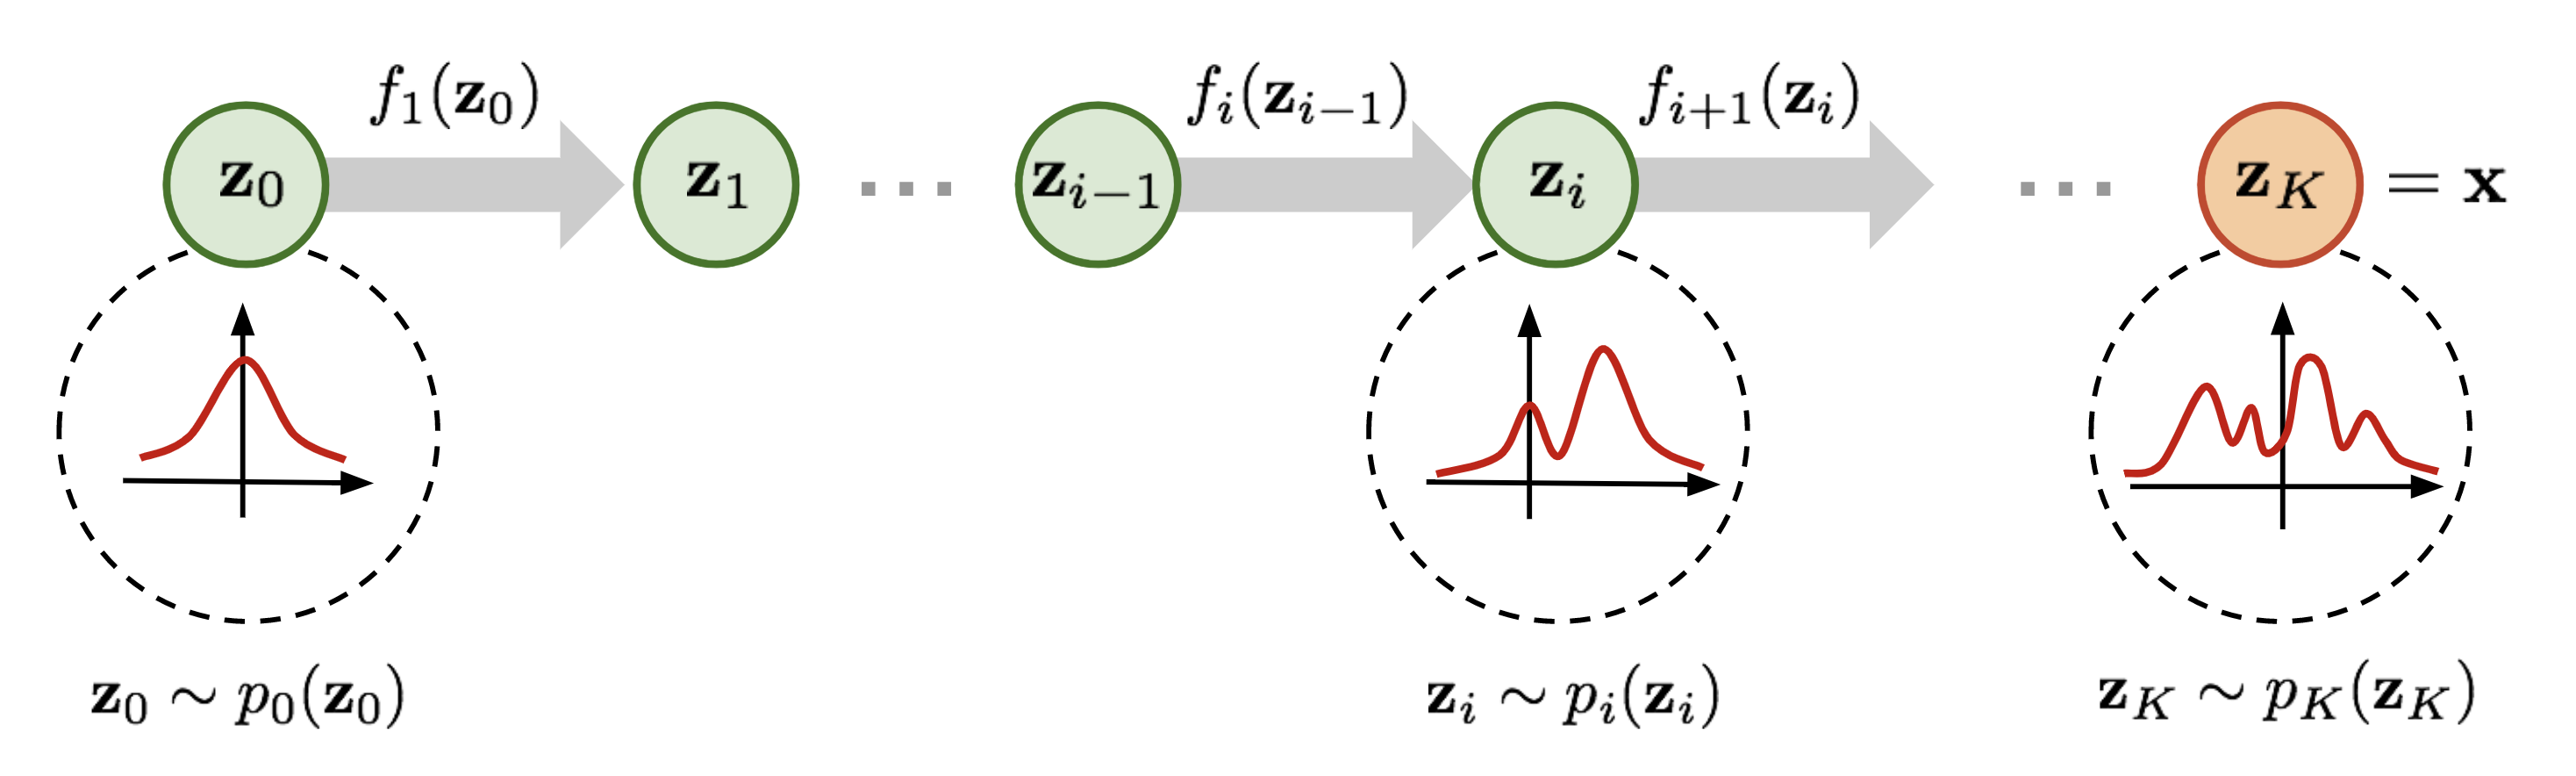
\includegraphics[width=\columnwidth]{gfx/ch4/normalizing-flow.png}
    \caption[Normalizing Flows]{The main idea behind Normalizing Flows: how can we find a chain of invertible transformations to send $p_z(\mathbf{z})$ to $p_x(\mathbf{x})$? Taken from \cite{nffig}.}
    \label{fig:nf}
\end{figure}
	
Based on this, the idea is to define some kind of measure, which can then be used as the objective function to minimize, to learn the optimal transformation \emph{f}.

\subsection{Loss functions}

As the idea is to leverage deep learning, we let our transformation \emph{f} depend on a set of parameters $\phi$, $f = f(\mathbf{x};\, \phi)$.
For the sake of completeness, we distinguish two main cases.

\paragraph{Forward KL Divergence}
Suppose that we have samples from the target distribution (or we are able to generate them), but we cannot evaluate the underlying pdf $p_x^*(\mathbf{x})$. This is precisely our case in HEP, with billions of available Monte Carlo data and no analytical pdf. Then, we may define as our loss function the \emph{forward Kullback-Leibler divergence} between the target distribution $p_x^*(\mathbf{x})$ and the flow-defined one $p_x(\mathbf{x}; \, \phi)$:

\[
\begin{aligned}
    \mathcal{L}(\phi) &= \mathcal{D}_{KL}[p_x^*(\mathbf{x})||p_x(\mathbf{x}; \, \phi)]\\
    &= -\mathbb{E}_{p_x^*(\mathbf{x})}[\log(p_x(\mathbf{x}; \, \phi))] +\; \text{const.}\\
    &= -\mathbb{E}_{p_x^*(\mathbf{x})}[\log(p_z(f^{-1}(\mathbf{x}; \, \phi)))+\log\left(\det\mathbb{J}_{f^{-1}}(\mathbf{x}; \, \phi)\right)] +\; \text{const.}
\end{aligned}
\]

where we have used Eq. \ref{eqn:logpdf}. Supposing we had a set of training samples $\{\mathbf{x}\}^N_n$ from the target pdf, we may estimate the expectation value over $p_x^*(\mathbf{x})$ by Monte Carlo as:

\[
\mathcal{L}(\phi) \approx -\frac{1}{N} \sum_n \log(p_z(f^{-1}(\mathbf{x}; \, \phi)))+\log\left(\det\mathbb{J}_{f^{-1}}(\mathbf{x}_n; \, \phi)\right) +\; \text{const.}
\]

For computing this loss we need to calculate $f^{-1}$, its Jacobian determinant and the density $p_z(f^{-1}(\mathbf{x}; \, \phi))$. 

\paragraph{Reverse KL Divergence} If instead we have the ability to easily evaluate $p_x^*(\mathbf{x})$ but not to sample from it, the \emph{reverse Kullback-Leibler divergence} is more well suited:

\[
\begin{aligned}
    \mathcal{L}(\phi) &= \mathbb{E}_{p_x(\mathbf{x}, \, \phi)}[\log(p_x(\mathbf{x}; \, \phi)) - \log(p_x^*(\mathbf{x}))]\\
    &= \mathbb{E}_{p_x(\mathbf{x}, \, \phi)}[\log(p_z(\mathbf{z}))-\log\left(\det\mathbb{J}_{f}(\mathbf{x}; \, \phi)\right)-\log(p_x(\mathbf{x}; \, \phi))]
\end{aligned}
\]

\section{Constructing flows}
For an actual implementation, the main challenge is in designing parametrizable multivariate bijections that have closed form expressions for both $f$ and $f^{-1}$, a tractable Jacobian whose calculation scales with $O(D)$ rather than $O(D^3)$, and can express a flexible class of functions.

\subsection{Coupling Layers}

One simple way to reduce the computational complexity of the Jacobian is to introduce \emph{coupling layers}. The basic idea is illustrated in Figure \ref{fig:coupla}.

\begin{figure}
    \centering
    \scalebox{0.65}{
    \begin{tikzpicture}[
        thick, node distance=15mm,
        set/.style={draw, diamond, text width=8mm, align=center},
        op/.style={draw, circle, text width=5mm, align=center, fill=orange!40},
      ]
    
      \node[set, fill=blue!20] (z1) {$\vec z_{1:d}$};
      \node[op, right=of z1] (eq) {\raisebox{-1ex}=};
      \node[set, right=of eq, fill=blue!20] (x1) {$\vec x_{1:d}$};
      \draw[->] (z1) edge (eq) (eq) edge (x1);
    
      \node[set, below=1 of z1, fill=green!30] (z2) {$\mathclap{\vec z_{d+1:D}}$};
      \node[op, right=of z2] (g) {$f$};
      \node[below=1em of g] (forward) {forward pass};
      \node[set, right=of g, fill=yellow!40] (x2) {$\mathclap{\vec x_{d+1:D}}$};
      \draw[->] (z2) edge (g) (g) edge (x2);
    
      \node[op] (m) at ($(z1)!0.5!(g)$) {$\phi$};
      \draw[->] (z1) edge (m) (m) edge (g);
    
      \begin{scope}[xshift=9cm]
    
        \node[set, fill=blue!20] (z1) {$\vec z_{1:d}$};
        \node[op, right=of z1] (eq) {\raisebox{-1ex}=};
        \node[set, right=of eq, fill=blue!20] (x1) {$\vec x_{1:d}$};
        \draw[<-] (z1) edge (eq) (eq) edge (x1);
    
        \node[set, below=1 of z1, fill=green!30] (z2) {$\mathclap{\vec z_{d+1:D}}$};
        \node[op, right=of z2] (g) {$\mathclap{f^{-1}}$};
        \node[below=1em of g] (inverse) {inverse pass};
        \node[set, right=of g, fill=yellow!40] (x2) {$\mathclap{\vec x_{d+1:D}}$};
        \draw[<-] (z2) edge (g) (g) edge (x2);
    
        \node[op] (m) at ($(x1)!0.5!(g)$) {$\phi$};
        \draw[->] (x1) edge (m) (m) edge (g);
    
      \end{scope}
    
    \end{tikzpicture}}
    \caption[Coupling layer]{The two possible passes through a coupling layer.}
    \label{fig:coupla}
\end{figure}

We partition the input $\mathbf{z} \in \mathbb{R}^D$ into two subsets $(\vec z_{1:d}, \, \vec z_{d+1:D}) \in \mathbb{R}^d \times \mathbb{R}^{D-d}$, where \emph{d} is an integer between 1 and \emph{D}, and is usually taken as $\lceil D/2 \rceil$. Then, at each step, the transformation $f_i$ is defined as:

\[
f_i(\mathbf{z}; \, \phi) = f_i(\vec z_{d+1:D}; \, \phi(\vec z_{1:d}))
\]

that is, the single transformation acts only on a \emph{subset} of the input, keeping the other part unchaged and using it as \emph{conditioning} for the actual parameters. 

At the end, the two subset are joined together to form the input for the next layer; by applying arbitrary permutations between the indexes we can ensure that eventually all values of the input get transformed. What is more, this also means that because we condition on the different indexes of the same input the transformation can correctly learn to model \emph{correlations} between 1d distribution for the same instance.

But the greatest advantage is that now the single transformation depends only on one subset of inputs, and thus its jacoban is \emph{block triangular}:

\[
\mathbb{J}_{f}(\mathbf{x}; \, \phi) = 
\begin{pmatrix}
\frac{\partial \vec x_{1:d}}{\partial \vec z_{1:d}} & \frac{\partial \vec x_{1:d}}{\partial \vec z_{d+1:D}}\\
\frac{\partial \vec x_{d+1:D}}{\partial \vec z_{1:d}} & \frac{\partial \vec x_{d+1:D}}{\partial \vec z_{d+1:D}}
\end{pmatrix}
=
\begin{pmatrix}
\mathbb{I} & 0\\
A & \mathbb{J}^*
\end{pmatrix}
\]

The full Jacobian determinant can simply be calculated from the product of the diagonal elements of $\mathbb{J}^*$, which are simply the partial derivatives over ($d+1, \dots D$). A similar reasoning holds for the Jacobian of the inverse.
This significantly speeds up the calculations.

\subsection{Splines}

There are many possible bijections which one can use in building a NF. Recent advancements have demonstrated the suitability of \emph{rational-quadratic spline transforms} (see \cite{durkan}). 

A monotonic spline is a piecewise function consisting of K segments, where each segment is a simple function that is easy to invert. Specifically, given a set of K+1 input locations $l_{0}, \dots, l_K$ , the transformation
is taken to be a simple monotonic function (e.g. a low-degree polynomial) in each interval
[$l_{k}, l_{k+1}$], under the constraint that the K segments meet at the endpoints.
Outside the interval [$l_{0}, l_K$], the transformer can default to a simple function such as the
identity. Typically, the parameters $\phi$ of the transformations are the input locations, 
the corresponding output locations and (depending on the type of spline) the
derivatives (i.e. slopes) at $l_{0}, \dots, l_K$. An example is illustrated in Figure \ref{fig:rqs}.

\begin{figure}
    \centering
    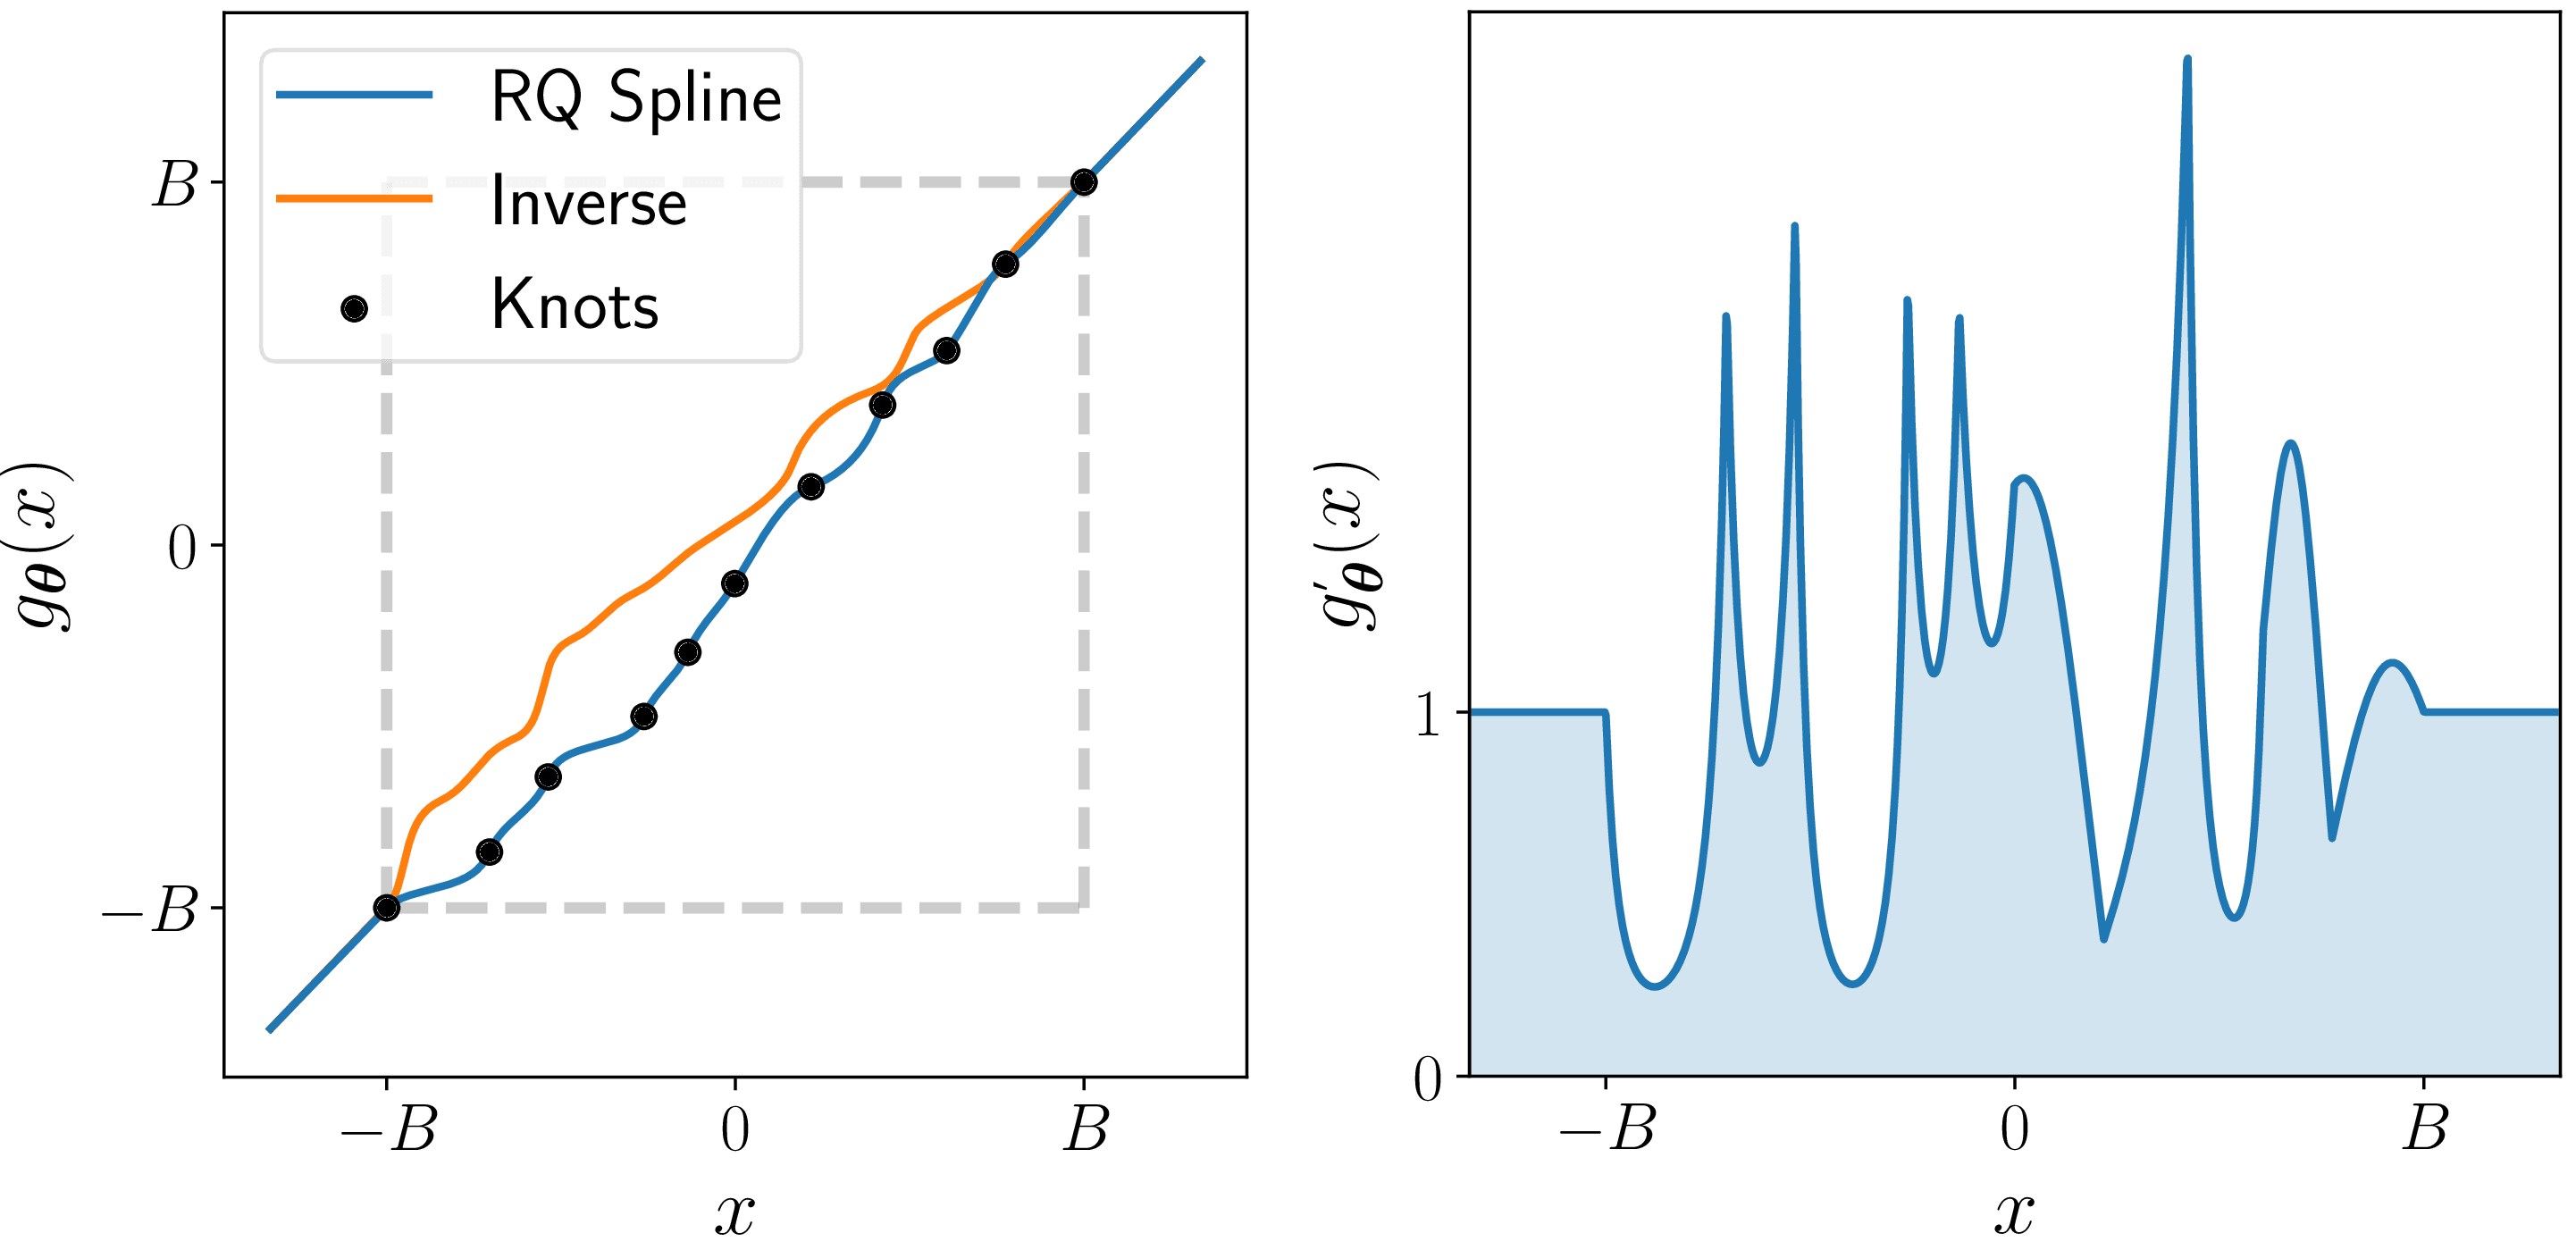
\includegraphics[width=\columnwidth]{gfx/ch4/D9F0PDyWsAAWKHf.png}
    \caption[Rational quadratic spline]{A rational quadratic spline $g_{\theta}(x)$ and its derivative $g_{\theta}^{'}(x)$}
    \label{fig:rqs}
\end{figure}

Spline-based transformers are as fast to invert as to evaluate, while
maintaining exact analytical invertibility. Evaluating or inverting a spline-based transformer
is done by first locating the right segment--which can be done in $\mathcal{O}$(log K) time using binary
search—and then evaluating or inverting that segment, which is assumed to be analytically
tractable. By increasing the number of segments K, a spline-based transformer can be
made arbitrarily flexible.

\subsection{Conditional distributions}

The theory of Normalizing Flows is also easily generalized to conditional distributions. We denote the variable to condition on by $C=\mathbf{c}\in\mathbb{R}^M$. A simple multivariate source of noise, for example a standard i.i.d. normal distribution, $\mathbf{z}\sim\mathcal{N}(\mathbf{0},I_{D\times D})$, is passed through a vector-valued bijection that also conditions on C, $f:\mathbb{R}^D\times\mathbb{R}^M\rightarrow\mathbb{R}^D$, to produce the more complex transformed variable $\mathbf{x}=f(\mathbf{z};\, \phi(C))$. 

In practice, this is usually accomplished by making the parameters for a known normalizing flow bijection $f$ the output of a neural network that inputs $\mathbf{c}$ as well as one of the subsets of the coupling layer. It is thus straightforward to condition event generation on some ground truth, e.g. the Monte Carlo Gen values matched to our targets.


\section{Applications}

Besides the generation of samples, the use cases of Normalzing Flows are numerous. 
Here we simply limit ourselves to those that we deem more interesting from a physicist point of view.

\paragraph{Density estimation and generation}

\paragraph{Inference}

\paragraph{Anomaly detection}
%*****************************************
%*****************************************
%*****************************************
%*****************************************
%*****************************************
